\documentclass[aspectratio=169, 9pt]{beamer}

% ==============================================================================
% THEME & NAVIGATION CONFIGURATION
% ==============================================================================
\usetheme[sectionpage=none]{metropolis}
\useoutertheme[subsection=false]{miniframes}
\nonstopmode

% ==============================================================================
% REQUIRED PACKAGES
% ==============================================================================
\usepackage{bookmark}
\usepackage{tikz}
\usetikzlibrary{shapes.geometric, arrows.meta, positioning, calc, shadows.blur}

\usepackage[utf8]{inputenc}
\usepackage[T1]{fontenc}
\usepackage{lmodern}
\usepackage{graphicx}
\graphicspath{{../assets/}{assets/}{templates/assets/}{../../templates/assets/}{./}}

\usepackage[backend=biber, style=numeric, sorting=none, maxnames=2, natbib=true, doi=false, url=false, isbn=false]{biblatex}
\addbibresource{references.bib}

\usepackage[most]{tcolorbox}
\usepackage{booktabs}
\usepackage{array}
\usepackage{colortbl}
\usepackage{listings}
\usepackage{amsmath, amssymb, amsfonts}

% ==============================================================================
% COLOR PALETTE (Editorial Crimson, Slate & Journal Navy)
% ==============================================================================
\definecolor{background}{RGB}{255, 255, 255}
\definecolor{foreground}{RGB}{30, 30, 40}
\definecolor{accent}{RGB}{220, 40, 40}
\definecolor{structure}{RGB}{50, 50, 60}
\definecolor{journalblue}{RGB}{26, 82, 118}
\definecolor{tableheader}{RGB}{240, 244, 248}

\setbeamercolor{normal text}{fg=foreground, bg=background}
\setbeamercolor{alerted text}{fg=accent}
\setbeamercolor{frametitle}{fg=foreground, bg=background}
\setbeamercolor{title separator}{fg=accent}
\setbeamercolor{section in head/foot}{fg=foreground, bg=structure!6}
\setbeamercolor{mini frame}{fg=accent, bg=structure!25}

\setbeamerfont{frametitle}{size=\large, series=\bfseries}
\setbeamerfont{title}{size=\Large, series=\bfseries}
\setbeamerfont{subtitle}{size=\normalsize}

% Progress Bar Header
\setbeamertemplate{headline}{%
  \begin{beamercolorbox}[wd=\paperwidth]{section in head/foot}
    \vskip3pt\centering
    \insertnavigation{0.7\paperwidth}%
    \vskip3pt%
  \end{beamercolorbox}%
  {\color{accent}\hrule height 2pt}%
}

% Minimalist Page Number Footer
\setbeamertemplate{footline}{%
  \vspace{3pt}%
  \hfill\usebeamercolor[fg]{page number in head/foot}\usebeamerfont{page number in head/foot}\insertframenumber\hspace*{1.2em}\vspace{3pt}%
}

% UI Helpers
\setbeamertemplate{itemize item}{\raisebox{0.18ex}{\textcolor{accent}{\rule{0.38em}{0.38em}}}}
\setbeamertemplate{itemize subitem}{\raisebox{0.15ex}{\textcolor{accent!60}{\rule{0.28em}{0.28em}}}}
\setlength{\labelsep}{0.5em}

\newtcbox{\pill}{on line, enhanced, colframe=accent, boxrule=0pt, arc=2.5pt,
  interior style={top color=accent, bottom color=accent!85},
  coltext=white, left=4pt, right=4pt, top=1.2pt, bottom=1.2pt,
  fontupper=\fontsize{6pt}{7pt}\selectfont\bfseries\sffamily}

\newtcbox{\pillalt}{on line, enhanced, colframe=structure, boxrule=0pt, arc=2.5pt,
  interior style={top color=structure!85, bottom color=structure!70},
  coltext=white, left=4pt, right=4pt, top=1.2pt, bottom=1.2pt,
  fontupper=\fontsize{6pt}{7pt}\selectfont\bfseries\sffamily}

\newtcolorbox{takeaway}[1][]{enhanced, colframe=accent, boxrule=0pt, leftrule=2.5pt,
  interior style={left color=accent!10, right color=accent!2},
  arc=1.5pt, outer arc=1.5pt, left=5pt, right=5pt, top=3pt, bottom=3pt,
  fontupper=\scriptsize, before skip=3pt, after skip=2pt, #1}

\newcommand{\kpicard}[3]{%
  \begin{tcolorbox}[enhanced, colframe=structure!20, colback=structure!3, boxrule=0.5pt, arc=2pt,
    left=3pt, right=3pt, top=2.5pt, bottom=2.5pt, halign=center]
    {\fontsize{6pt}{7pt}\selectfont\bfseries\textcolor{structure}{#1}}\\[1pt]
    {\normalsize\bfseries\textcolor{accent}{#2}}\\[1pt]
    {\tiny\textcolor{structure!70}{#3}}
  \end{tcolorbox}%
}

% ==============================================================================
% PRESENTATION METADATA
% ==============================================================================
\title{Probability Theory and Statistical Inference}
\subtitle{Axiomatic Foundations, Limit Theorems, Density Modeling, and Association Tests}
\author{Prof.~Alex Morgan \and Dr.~Jordan Taylor}
\institute{Department of Statistics \& Mathematical Sciences}
\date{\today}

\setbeamertemplate{title page}{
  \vfill
  \centering
  
\includegraphics[height=1.3cm]{university_seal.jpg}\par\vspace{0.4em}
  \usebeamerfont{title}\inserttitle\par
  \vspace{0.2em}
  \usebeamerfont{subtitle}\textcolor{structure}{\insertsubtitle}\par
  \vspace{0.5em}
  {\color{accent}\rule{0.75\textwidth}{1.2pt}}\par
  \vspace{0.5em}
  \usebeamerfont{author}\insertauthor\par
  \vspace{0.2em}
  \usebeamerfont{institute}\textcolor{structure!75}{\insertinstitute}\par
  \vspace{0.2em}
  \usebeamerfont{date}\textcolor{structure!55}{\insertdate}\par
  \vfill
}

% ==============================================================================
% DOCUMENT BEGIN
% ==============================================================================
\begin{document}

% --- Slide 1: Title ---
\begin{frame}[plain]
    \titlepage
\end{frame}

% --- Slide 2: Roadmap ---
\section{Roadmap}
\begin{frame}{Statistical Inquiry Roadmap}
    \begin{columns}[c]
        \begin{column}{0.48\textwidth}
            \pillalt{CURRICULUM}\par\vspace{0.3em}
            \begin{itemize}\setlength{\itemsep}{2.5pt}
                \item \textbf{1. Probability Axioms:} Conditional spaces and Bayes' rule~\cite{feller1968introduction}.
                \item \textbf{2. Random Moments:} Expectations, variance, and covariances.
                \item \textbf{3. Asymptotic Limit Theorems:} LLN and Central Limit Theorem.
                \item \textbf{4. Density Modeling:} Gaussian distribution and empirical rule.
                \item \textbf{5. Categorical Association:} Contingency tables and $\chi^2$ tests~\cite{casella2002statistical}.
            \end{itemize}
        \end{column}
        \begin{column}{0.48\textwidth}
            \begin{takeaway}
                \textbf{\textcolor{accent}{Core Objective:}} Formulate exact probability models and derive sample estimators with known asymptotic distributions.
            \end{takeaway}
            \vspace{0.4em}
            \begin{columns}[c]
                \begin{column}{0.48\textwidth}
                    \kpicard{SAMPLE SIZE}{$N = 1{,}200$}{Cohort Total}
                \end{column}
                \begin{column}{0.48\textwidth}
                    \kpicard{CONFIDENCE}{$95.0\%$}{Coverage Interval}
                \end{column}
            \end{columns}
        \end{column}
    \end{columns}
\end{frame}

% --- Slide 3: Probability Axioms & Bayes' Rule ---
\section{Probability}
\begin{frame}{Probability Axioms \& Bayesian Inversion}
    \begin{columns}[t]
        \begin{column}{0.48\textwidth}
            \pillalt{AXIOMATIC SPACE}\par\vspace{0.2em}
            \scriptsize
            Let $(\Omega, \mathcal{F}, P)$ be a probability space.
            \begin{itemize}\setlength{\itemsep}{2pt}
                \item \textbf{Non-negativity:} $P(A) \ge 0 \quad \forall A \in \mathcal{F}$.
                \item \textbf{Total Mass:} $P(\Omega) = 1$.
                \item \textbf{Countable Additivity:} $P\left(\bigcup_{i=1}^\infty A_i\right) = \sum_{i=1}^\infty P(A_i)$ for disjoint $A_i$.
            \end{itemize}
            \vspace{0.2em}
            \textbf{Conditional Probability:}
            \begin{equation*}
                P(A \mid B) = \frac{P(A \cap B)}{P(B)}, \quad P(B) > 0
            \end{equation*}
        \end{column}
        \begin{column}{0.48\textwidth}
            \pill{BAYES' THEOREM}\par\vspace{0.2em}
            \scriptsize
            Let $\{B_1, \dots, B_k\}$ partition $\Omega$:
            \begin{equation*}
                P(B_i \mid A) = \frac{P(A \mid B_i) P(B_i)}{\sum_{j=1}^k P(A \mid B_j) P(B_j)}
            \end{equation*}
            \vspace{0.1em}
            \begin{itemize}\setlength{\itemsep}{2pt}
                \item \textbf{Prior $P(B_i)$:} Baseline belief before observation.
                \item \textbf{Likelihood $P(A \mid B_i)$:} Evidence generation probability.
                \item \textbf{Posterior $P(B_i \mid A)$:} Updated belief given evidence $A$.
            \end{itemize}
            \vspace{0.2em}
            \begin{takeaway}
                \textbf{Key Takeaway:} Bayes' rule inverts conditional dependencies to infer latent parameters from observable data.
            \end{takeaway}
        \end{column}
    \end{columns}
\end{frame}

% --- Slide 4: Moments & Central Limit Theorem ---
\section{Asymptotics}
\begin{frame}{Random Moments \& The Central Limit Theorem}
    \begin{columns}[t]
        \begin{column}{0.48\textwidth}
            \pillalt{MOMENT OPERATORS}\par\vspace{0.2em}
            \scriptsize
            \textbf{1. Expected Value (First Moment):}
            \begin{equation*}
                \mathbb{E}[X] = \int_{-\infty}^{\infty} x f(x) \, dx
            \end{equation*}
            \textbf{2. Variance (Second Central Moment):}
            \begin{equation*}
                \mathrm{Var}(X) = \mathbb{E}[(X - \mu)^2] = \mathbb{E}[X^2] - (\mathbb{E}[X])^2
            \end{equation*}
            \textbf{3. Covariance Matrix:}
            \begin{equation*}
                \mathrm{Cov}(X, Y) = \mathbb{E}[(X - \mu_X)(Y - \mu_Y)]
            \end{equation*}
        \end{column}
        \begin{column}{0.48\textwidth}
            \pill{LIMIT CONVERGENCE}\par\vspace{0.2em}
            \scriptsize
            \textbf{Lindeberg-L\'{e}vy Central Limit Theorem:}
            For i.i.d. $X_1, \dots, X_n$ with mean $\mu$ and variance $\sigma^2 < \infty$:
            \begin{equation*}
                Z_n = \frac{\bar{X}_n - \mu}{\sigma / \sqrt{n}} \xrightarrow{d} \mathcal{N}(0, 1) \quad \text{as } n \to \infty
            \end{equation*}
            \vspace{0.1em}
            \begin{itemize}\setlength{\itemsep}{2pt}
                \item \textbf{Weak Law (WLLN):} $\bar{X}_n \xrightarrow{p} \mu$.
                \item \textbf{Rate of Convergence:} Sampling error shrinks at parametric rate $\mathcal{O}(n^{-1/2})$.
            \end{itemize}
        \end{column}
    \end{columns}
\end{frame}

% --- Slide 5: Gaussian Distribution & Rejection Regions ---
\section{Inference}
\begin{frame}{Standard Normal Distribution \& Hypothesis Rejection}
    \begin{columns}[c]
        \begin{column}{0.44\textwidth}
            \pillalt{DENSITY MODEL}\par\vspace{0.2em}
            \scriptsize
            Standard Normal Density:
            \begin{equation*}
                \phi(z) = \frac{1}{\sqrt{2\pi}} \exp\left(-\frac{z^2}{2}\right)
            \end{equation*}
            \vspace{0.1em}
            \begin{itemize}\setlength{\itemsep}{1.5pt}
                \item \textbf{Empirical Rule (68-95-99.7):}
                \begin{itemize}\setlength{\itemsep}{1pt}
                    \item $P(|Z| \le 1) = 68.27\%$
                    \item $P(|Z| \le 2) = 95.45\%$
                    \item $P(|Z| \le 3) = 99.73\%$
                \end{itemize}
                \item \textbf{Type I Error Threshold ($\alpha = 0.05$):}
                Two-tailed critical values $z_{\mathrm{crit}} = \pm 1.96$.
                \item \textbf{Two-Tailed $p$-Value:}
                $p = 2 \cdot [1 - \Phi(|z_{\mathrm{stat}}|)]$.
            \end{itemize}
        \end{column}
        \begin{column}{0.54\textwidth}
            \centering
            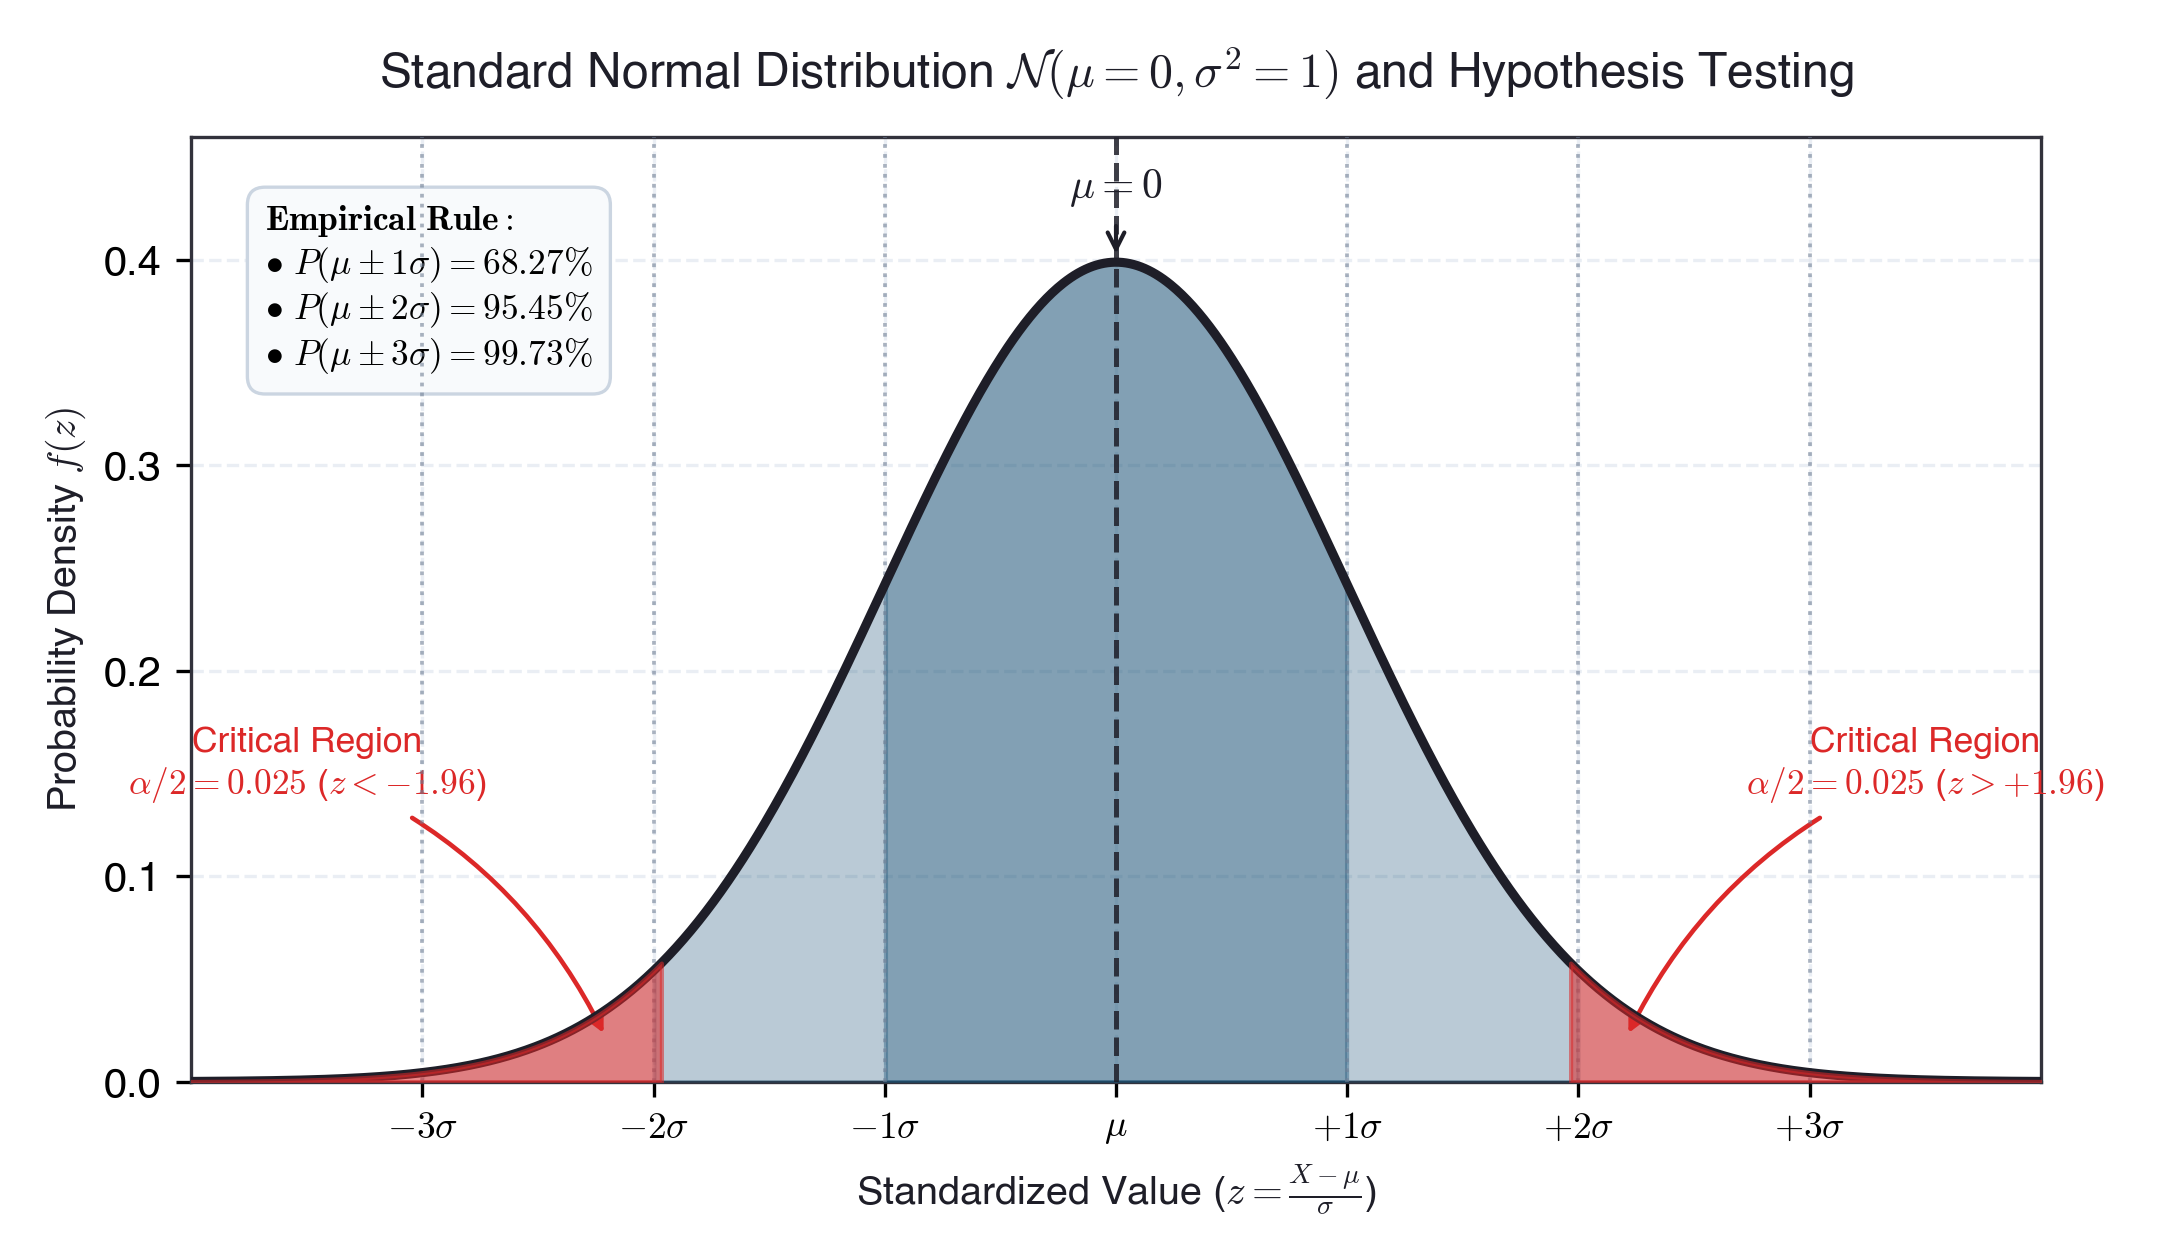
\includegraphics[width=\linewidth, height=0.68\textheight, keepaspectratio]{gaussian_distribution.png}\\[2pt]
            {\tiny\textcolor{structure!70}{Fig 1: High-DPI Python/Seaborn Standard Normal simulation with rejection regions.}}
        \end{column}
    \end{columns}
\end{frame}

% --- Slide 6: Contingency Tables & Chi-Square Tests ---
\section{Categorical}
\begin{frame}{Contingency Matrices \& Pearson's $\chi^2$ Test}
    \begin{columns}[c]
        \begin{column}{0.52\textwidth}
            \centering
            \setlength{\tabcolsep}{4.5pt}
            \scriptsize
            \begin{tabular}{@{} l c c c @{}}
                \toprule
                \rowcolor{tableheader}
                \textbf{Cohort Group} & \textbf{Outcome ($Y=1$)} & \textbf{Control ($Y=0$)} & \textbf{Total ($R_i$)} \\
                \midrule
                Treatment ($D=1$)  & $n_{11} = 420$          & $n_{12} = 180$          & $600$ \\
                Control ($D=0$)    & $n_{21} = 210$          & $n_{22} = 390$          & $600$ \\
                \midrule
                \textbf{Total ($C_j$)} & $630$              & $570$              & $N = 1{,}200$ \\
                \bottomrule
            \end{tabular}
            \par\vspace{4pt}
            {\tiny\textcolor{structure!70}{Cross-tabulation of sample cohorts with marginal frequencies.}}
            \vspace{0.4em}
            \begin{takeaway}
                \textbf{Decision:} $\chi^2_{\mathrm{calc}} = 147.37 \gg \chi^2_{0.05, 1} = 3.84 \implies \text{Reject } H_0$ ($p < 0.001$).
            \end{takeaway}
        \end{column}
        \begin{column}{0.46\textwidth}
            \pillalt{TEST FORMULATION}\par\vspace{0.2em}
            \scriptsize
            \begin{itemize}\setlength{\itemsep}{2pt}
                \item \textbf{Expected Frequency ($E_{ij}$):}
                \begin{equation*}
                    E_{ij} = \frac{R_i \times C_j}{N}
                \end{equation*}
                \item \textbf{Pearson's $\chi^2$ Statistic:}
                \begin{equation*}
                    \chi^2 = \sum_{i=1}^r \sum_{j=1}^c \frac{(O_{ij} - E_{ij})^2}{E_{ij}} \sim \chi^2_{(r-1)(c-1)}
                \end{equation*}
                \item \textbf{Sample Odds Ratio ($\widehat{\mathrm{OR}}$):}
                \begin{equation*}
                    \widehat{\mathrm{OR}} = \frac{n_{11} n_{22}}{n_{12} n_{21}} = \frac{420 \times 390}{180 \times 210} = 4.33
                \end{equation*}
            \end{itemize}
        \end{column}
    \end{columns}
\end{frame}

% --- Slide 7: Python Code Listing ---
\begin{frame}[fragile]{Statistical Estimation in Python}
\begin{lstlisting}[language=Python, basicstyle=\ttfamily\scriptsize, keywordstyle=\color{accent}\bfseries, commentstyle=\color{structure!60}\itshape, stringstyle=\color{journalblue}, frame=single, rulecolor=\color{structure!20}, backgroundcolor=\color{structure!3}, numbers=left, numberstyle=\tiny\color{structure!50}]
import numpy as np
from scipy import stats

def perform_contingency_analysis(table: np.ndarray):
    """Computes Chi-Square statistic, p-value, and Odds Ratio."""
    chi2, p_val, dof, expected = stats.chi2_contingency(table, correction=False)
    
    # 2x2 Odds Ratio calculation
    a, b = table[0, 0], table[0, 1]
    c, d = table[1, 0], table[1, 1]
    odds_ratio = (a * d) / (b * c)
    se_ln_or = np.sqrt(1/a + 1/b + 1/c + 1/d)
    ci_95 = np.exp(np.log(odds_ratio) + np.array([-1, 1]) * 1.96 * se_ln_or)
    
    return {"chi2": chi2, "p_value": p_val, "odds_ratio": odds_ratio, "ci_95": ci_95}
\end{lstlisting}
\end{frame}

% --- Slide 8: Summary ---
\section{Summary}
\begin{frame}{Key Statistical Takeaways}
    \begin{columns}[t]
        \begin{column}{0.48\textwidth}
            \pill{SUMMARY}\par\vspace{0.3em}
            \begin{itemize}\setlength{\itemsep}{2.5pt}
                \item \textbf{Axiomatic Rigor:} Invert conditional probabilities via Bayes' rule.
                \item \textbf{CLT Asymptotics:} Normality emerges regardless of underlying distribution.
                \item \textbf{Categorical Testing:} $\chi^2$ tests evaluate independence against random marginal allocation.
            \end{itemize}
        \end{column}
        \begin{column}{0.48\textwidth}
            \pillalt{NEXT STEPS}\par\vspace{0.3em}
            \begin{itemize}\setlength{\itemsep}{2.5pt}
                \item \textbf{Problem Set 1:} Derive the CLT for exponential distributions.
                \item \textbf{Lab 1:} Simulate empirical coverage of $\widehat{\mathrm{OR}}$ confidence intervals.
                \item \textbf{Office Hours:} Tuesday 10:00--12:00 (Math Hall 302).
            \end{itemize}
            \vspace{0.3em}
            \begin{takeaway}
                \textbf{Contact:} \texttt{stat-instructor@university.edu}
            \end{takeaway}
        \end{column}
    \end{columns}
\end{frame}

% --- Slide 9: References ---
\begin{frame}[allowframebreaks]{References}
    \printbibliography
\end{frame}

\end{document}
